\subsection{Língua Mura}

\begin{questions}
\question{
Foi encontrada uma nova língua da família linguística mura,
falada em uma aldeia de pouco mais de 100 indígenas nas proximidades
do rio Madeira, no Amazonas. 
Esta língua falada por um povo semi-nômade é bem parecida com o pirarrã.
A língua é bem simples em seu repertório fonêmico, constituído de apenas
3 vogais e 3 consoantes: /i/, /a/, /u/, /p/, /t/, /k/. 
Linguistas construíram um corpus para esta língua e verificaram que
os fonemas apresentam a seguinte distribuição $p = (6/21, 5/21, 4/21, 3/21, 2/21, 1/21)$.
Verificou-se ainda que esta língua possui ainda duas formas escritas fonêmica:
\begin{inlineenum}
\item uma forma que utiliza um alfabeto com dois símbolos ($\sqcap$ e $\wedge$);
\item e outra que utiliza um alfabeto com três símbolos ($\dagger$, $\ddagger$ e $\times$).
\end{inlineenum}
Ambos códigos utilizados por esta tribo surpreenderam os cientistas ao verificarem
que se tratavam de códigos ótimo de prefixo.

\begin{parts}
\part Encontre ambos os códigos utilizados e faça uma tabela para representar cada uma deles.

\part Calcule o comprimento esperado de cada um dos códigos.

\part Seja $X$ uma variável aleatória que representa os fonemas naquela língua,
calcule a entropia de $X$.

\part Compare os valores encontrados e explique o que você pode observar através desta comparação.
É possível melhorar a eficiência deste código? Explique como.

\end{parts}
}

\begin{solution}
\begin{parts}
\part 
Se as tribos utilizam códigos ótimo de prefixo, podemos concluir que trata-se de
um código de Huffmann. Devemos então achar um código de Huffmann 
\begin{inlineenum}
\item binário;
\item e ternário.
\end{inlineenum}

\begin{minipage}[b]{0.6\textwidth}
\tikzset{every tree node/.style={align=left,anchor=north,minimum width=2em,draw,circle},
         blank/.style={draw=none},
         edge from parent/.style=
         {draw, edge from parent path={(\tikzparentnode) -- (\tikzchildnode)}},
         every node/.append style={align=left},
         level distance=1.2cm}
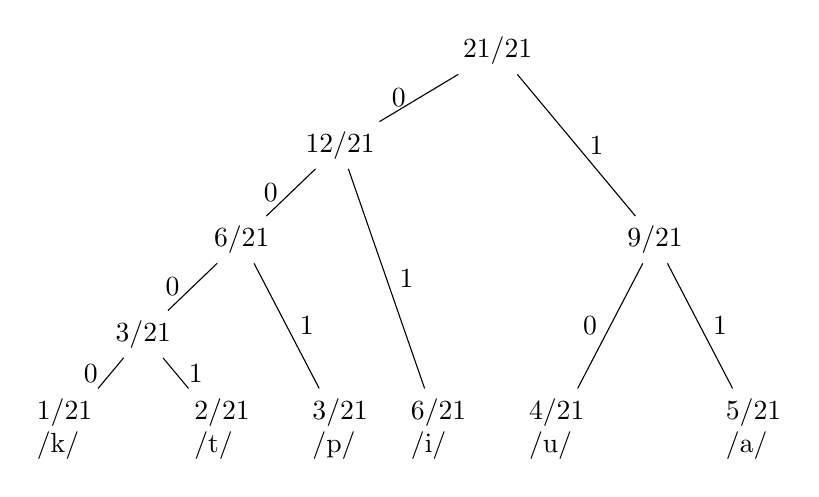
\begin{tikzpicture}[level distance=1.2cm,
  level 1/.style={sibling distance=4cm},
  level 2/.style={sibling distance=2.5cm},
  level 3/.style={sibling distance=2.5cm},
  level 4/.style={sibling distance=2.0cm},
  level 5/.style={sibling distance=1.5cm},
  % Skip a level in the tree
    skip level/.default={1},
    skip level/.style={
        level distance=\tikzleveldistance*#1+\tikzleveldistance},
    skip level spaced/.default={1},
    skip level spaced/.style={
        skip level=#1,
        sibling distance=\tikzsiblingdistance*#1+\tikzsiblingdistance},
  % code on edge:
    code/.style={
        insert path={edge from parent node[code label] {$#1$}}},
    code label/.style={outer sep=.5mm},
]
  \node {21/21}
  child { node {12/21} 
          child {
                node {6/21} 
                child {
                        node {3/21}
                        child { node {1/21 \\ /k/} [left, code=0]}
                        child { node {2/21 \\ /t/} [right, code=1]}
                        [left, code=0]
                }
                child[skip level=1] {
                        node {3/21 \\ /p/}
                        [right, code=1]
                }
                [left, code=0]
         }
        child[skip level=2] { node {6/21 \\ /i/} [right, code=1]}
        [left, code=0]
  }
  child[skip level=1] { 
        node {9/21}
        child { node {4/21 \\ /u/} [left, code=0]} 
        child { node {5/21 \\ /a/} [right, code=1]}
        [right, code=1] 
  };
\end{tikzpicture}
\end{minipage}
  \hfill
\begin{minipage}[b]{0.35\textwidth}
   %\vspace{-3em}
        % ($\sqcap$ e $\wedge$)
   \begin{center}
   \begin{tabular}[b]{clc}
        $x$ & $C(x)$ & $l(x)$ \\
        /i/ & 01  & 2 \\
        /a/ & 11  & 2 \\
        /u/ & 10  & 2 \\
        /p/ & 001 & 3 \\
        /t/ & 0001 & 4 \\
        /k/ & 0000 & 4
   \end{tabular}
   \end{center}

   \ \\
   Comprimento esperado:
   \begin{eqnarray}
   L(C) &=& \sum_x p(x) l(x) = \nonumber \\
        &=& \frac{17}{7} = 2.43  .
   \end{eqnarray}

   Entropia:
   \begin{eqnarray}
   H(X) &=& - \sum_x p(x) \log p(x) \nonumber \\ 
        &=& \log 7 - \frac{5}{21} \log 5 + \nonumber \\
	    && \frac{12}{21} \log 3 - \frac{16}{21} \nonumber \\
        &=& 2.3983 \text{ bits} .
   \end{eqnarray}
\end{minipage}

No Octave:
\begin{lstlisting}[language=Octave]
pkg load communications
p = [6/21, 5/21, 4/21, 3/21, 2/21, 1/21];
h = huffmandict({'i','a','u','p','t','k'},p);
\end{lstlisting}



\begin{minipage}[b]{0.6\textwidth}
\tikzset{every tree node/.style={align=left,anchor=north,minimum width=2em,draw,circle},
         blank/.style={draw=none},
         edge from parent/.style=
         {draw, edge from parent path={(\tikzparentnode) -- (\tikzchildnode)}},
         every node/.append style={align=left},
         level distance=1.5cm}
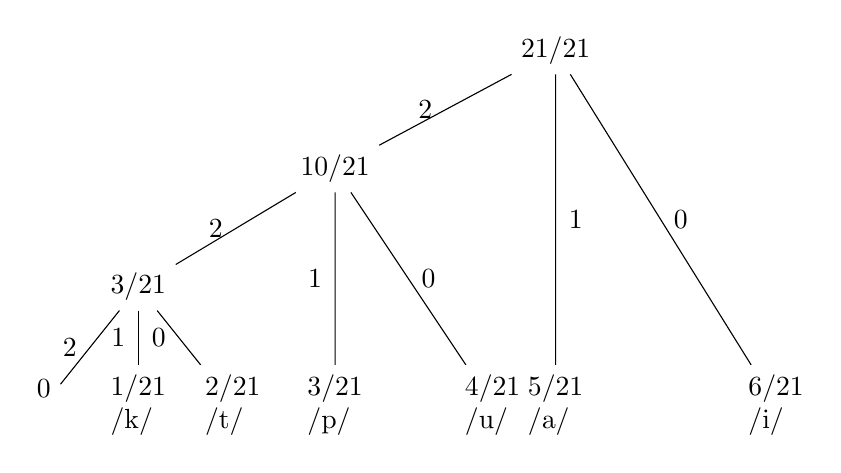
\begin{tikzpicture}[level distance=1.5cm,
  level 1/.style={sibling distance=2.8cm},
  level 2/.style={sibling distance=2.5cm},
  level 3/.style={sibling distance=1.2cm},
  % Skip a level in the tree
    skip level/.default={1},
    skip level/.style={
        level distance=\tikzleveldistance*#1+\tikzleveldistance},
    skip level spaced/.default={1},
    skip level spaced/.style={
        skip level=#1,
        sibling distance=\tikzsiblingdistance*#1+\tikzsiblingdistance},
  % code on edge:
    code/.style={
        insert path={edge from parent node[code label] {$#1$}}},
    code label/.style={outer sep=.5mm},
]
  \node {21/21}
  child {
        node {10/21}
        child { node {3/21} 
                child { node {0 \\ $\square$ } [left, code=2]  }
                child { node {1/21 \\ /k/} [left, code=1]  }
                child { node {2/21 \\ /t/} [left, code=0]  }
                [left, code=2]
        }
        child[skip level=1] { node {3/21 \\ /p/} [left, code=1]  }
        child[skip level=1] { node[xshift=-0.5cm] {4/21 \\ /u/} [right, code=0] }
        [left, code=2]
  }
  child[skip level=2] {
        node {5/21 \\ /a/} [right, code=1]
  }
  child[skip level=2] {
        node {6/21 \\ /i/} [right, code=0]
  };
\end{tikzpicture}
\end{minipage}
  \hfill
\begin{minipage}[b]{0.35\textwidth}
   \begin{center}
   \begin{tabular}[b]{clc}
        $x$ & $C(x)$ & $l(x)$ \\
        /i/ & 0    & 1 \\
        /a/ & 1    & 1 \\
        /u/ & 20   & 2 \\
        /p/ & 21   & 2 \\
        /t/ & 220  & 3 \\
        /k/ & 221  & 3
   \end{tabular}
   \end{center}

   \ \\
   Comprimento esperado:
   \begin{equation}
   L(C) = \sum_x p(x) l(x) = 1.619 .
   \end{equation}


   Entropia:
   \begin{eqnarray}
   H(X) &=& - \sum_x p(x) \log p(x) \nonumber \\ 
        &=& 2.3983 \text{ bits} \nonumber \\
        &=& \frac{1}{\log_2 3} H_2(X) \text{ trits} \nonumber \\
        &=& 1.5132 \text{ trits} .
   \end{eqnarray}
\end{minipage}

\begin{lstlisting}[language=Octave]
p = [1:6]/21;
l = [3, 3, 2, 2, 1, 1];

function H=entropy(p,b)
if nargin < 2, b=2; endif;
H = (-sum(p.*log2(p)))/(log2(b));
endfunction

>> entropy(p,2)
ans =  2.3983
>> entropy(p,3)
ans =  1.5132
\end{lstlisting}

Observe que em todos os casos temos $L > H$, respeitando assim o limite de Shannon ($L \geq H$).
Apesar de $L$ já ser próximo de $H$, é possível ainda aproximar mais do limite de Shannon,
para tanto é necessário realizar a codificação em blocos ou em fluxo. O código de Huffmann é ótimo,
dentre os códigos de símbolos, ou seja, fornece o menor $L$ dentre os códigos para símbolos, desta
forma os comprimentos das palavras serão inteiros. O código de Huffmann atingirá exatamente o limite
quando a distribuição for d-ádica, o que não é o caso.


\end{parts}
\end{solution}
\end{questions}

